\documentclass[11pt,a4paper]{article}
\usepackage[top=0.8in,bottom=0.8in,left=1.2in,right=0.6in]{geometry}
\usepackage[utf8]{inputenc}
\usepackage{ctex}
%\usepackage{assignpkg}
\usepackage{xltxtra}
\usepackage[colorlinks,linkcolor=red]{hyperref}
\usepackage{float}
\usepackage{color}
\usepackage{fontspec}
\usepackage{amsmath}
\usepackage{xcolor}
\setCJKmonofont{KaiTi}
\setmainfont[BoldFont={SimHei},ItalicFont={KaiTi}]{SimSun}
\setsansfont[BoldFont=SimHei]{KaiTi}
\setmonofont{NSimSun}
\XeTeXlinebreaklocale "zh"
\XeTeXlinebreakskip = 0pt plus 1pt minus 0.1pt
\usepackage{listings}

\lstset{
	language=C++,
	basicstyle={\ttfamily},
	numbers=left,
	keywordstyle=\color{blue},
	numberstyle={\tiny\color{lightgray}},
	stepnumber=1, %行号会逐行往上递增
	numbersep=5pt,
	commentstyle=\small\color{red},
	backgroundcolor=\color[rgb]{0.95,1.0,1.0},
	showspaces=false,
	showtabs=false,
	frame=shadowbox, framexleftmargin=5mm, 
	rulesepcolor=\color{red!20!green!20!blue!20!},
	% frame=single,
	%  TABframe=single,
	tabsize=4,
	breaklines=tr,
	escapeinside=``,
	extendedchars=false %这一条命令可以解决代码跨页时,章节标题,页眉等汉字不显示的问题
}
\usepackage{setspace}
\setlength{\parindent}{0pt} %取消缩进
%\studentIds{网络空间安全}{胡孟}
%\studentNames{专业}{姓名}

%\assignmentNumber{1}
\newcommand{\sanhao}{\fontsize{16pt}{24pt}\selectfont}  
\begin{document}
{\bfseries \kaishu \sanhao \begin{center}
		{\huge $\textbf{暨南大学本科实验报告专用纸\quad }$}
\end{center}}
%\makecover
\begin{spacing}{1.7}
{\Large {\kaishu 课程名称\underline{\quad\qquad\qquad 计算机网络实验\qquad\qquad\quad }}{\kaishu 成绩评定\underline{\qquad\qquad}}}

{\Large {\kaishu 实验项目名称\underline{\qquad\;\,  TCP与UDP端口扫描 \quad\;}指导老师\underline{\;\; 某某某\;\;\:}}}

{\Large{\kaishu 实验项目编号\underline{\quad9\quad}实验项目类型\underline{\quad 综合类\quad}实验地点\underline{\quad\:\:\:\:N117\quad}}}

{\Large {\kaishu 学生姓名\underline{\qquad\qquad 某某\qquad\qquad}学号\underline{\qquad\qquad xxxxxxxxxx\qquad\qquad}}}

{\Large {\kaishu 学院\underline{\qquad 网络空间安全学院\qquad}系\underline{\qquad}专业\underline{\qquad 网络空间安全\quad\:\:}}}

{\Large {\kaishu 实验时间\underline{\:\:2020\:\:}\!\:年\underline{\:\;12\:\;}\!\:月\underline{\:9\:}\!\:日\underline{\:\:晚\:\:}\!\:上\!\:$\sim$\!\:\underline{\:\:2020\:\:}\!\:年\underline{\:\;12\:\;}\!\:月\underline{\:\:9\:\:}\!\:日\underline{\:晚\:}\!\:上}}
\end{spacing}

\section*{(一)实验目的}
\begin{itemize}
	\item[1.] {\large 了解常用的TCP、UDP端口扫描的原理及其各种手段}
	\item[2.] {\large 增强网络安全意识}
\end{itemize}

\section*{(二)实验环境}
\qquad{\large 该实验采用网络结构一}

\section*{(三)实验原理}


\section*{(四)实验步骤}

\section*{(五)实验结果与分析}

\section*{(六)附录}
基于Linux提供的网络编程API实现三种端口扫描。为了加快扫描速度,可考虑创建多个线程进行并发扫描(这里指实现简易版)。
\newpage
{\bfseries \kaishu \sanhao \begin{center}
		{\huge $\textbf{暨南大学本科实验报告专用纸}$}{\Large $\textbf{(附页)\qquad}$}
\end{center}}
\rule[8pt]{15.5cm}{0.05em}
\qquad\\
\qquad\\
首先先随机生成5个50000$\sim$60000的数字作为端口号,绑定套接字,监听对应的端口。以下为TCP端口代码如下:
\begin{lstlisting}[language=C]
#include<stdio.h>
#include<stdlib.h>
#include<string.h>
#include<sys/socket.h>
#include<sys/types.h>
#include<arpa/inet.h>
#include<time.h>

int main(void){
    srand(time(NULL));
    int open_ports[5];
    int sockfds[5];
    int flag=1;
    for(int i=0; i<5; ++i){
        /*这里假设生成的随机数不重复(概率很小)*/
        open_ports[i] = rand()%10000 + 50000;
        sockfds[i] = socket(AF_INET,SOCK_STREAM,0);
        struct sockaddr_in servaddr;
        bzero(&servaddr,sizeof(servaddr));
        servaddr.sin_family = AF_INET;
        servaddr.sin_port = htons(open_ports[i]);
        servaddr.sin_addr.s_addr = htonl(INADDR_ANY);

        /*设置端口复用,使得处于time_wait状态的连接地址能重新绑定,便于实验*/
        setsockopt(sockfds[i],SOL_SOCKET,SO_REUSEADDR,&flag,sizeof(flag));

        bind(sockfds[i],(struct sockaddr*)&servaddr,sizeof(servaddr));
        listen(sockfds[i],5);      
    }
    for(int i=0; i<5; ++i){
        printf("listen port: %d\n",open_ports[i]);
    }
    while(1);
}
\end{lstlisting}
\begin{center}
TCP Connect端口扫描
\end{center}
这种扫描方法其实实现非常简单,只需要模拟客户端对目标主机做一次三次连接活动即可,检查connect返回值。为了突出整体逻辑,省去了部分检错代码。
\begin{lstlisting}[language=C]
#include<netinet/in.h>
#include<arpa/inet.h>
#include<unistd.h>
#include<stdio.h>
#include<string.h>
#include<stdlib.h>

int main(int argc, char **argv)
{
    int sockfd, n;
    struct sockaddr_in servaddr;

    int i;
    for (i = atoi(argv[2]); i < atoi(argv[3]); i++) {
        sockfd = socket(AF_INET, SOCK_STREAM, 0);

        bzero(&servaddr, sizeof(servaddr));
        servaddr.sin_family = AF_INET;
        servaddr.sin_port = htons(i);
        inet_pton(AF_INET, argv[1], &servaddr.sin_addr);

        /*每次检查connect函数的返回值即可*/
        if (connect(sockfd, (struct sockaddr*) &servaddr, sizeof(servaddr)) < 0) {
            close(sockfd);
        }
        else {
            printf("useful port: %d\n", i);
            close(sockfd);
        }
    }
    return 0; 
}
\end{lstlisting}
\begin{figure}[H]
    \centering
    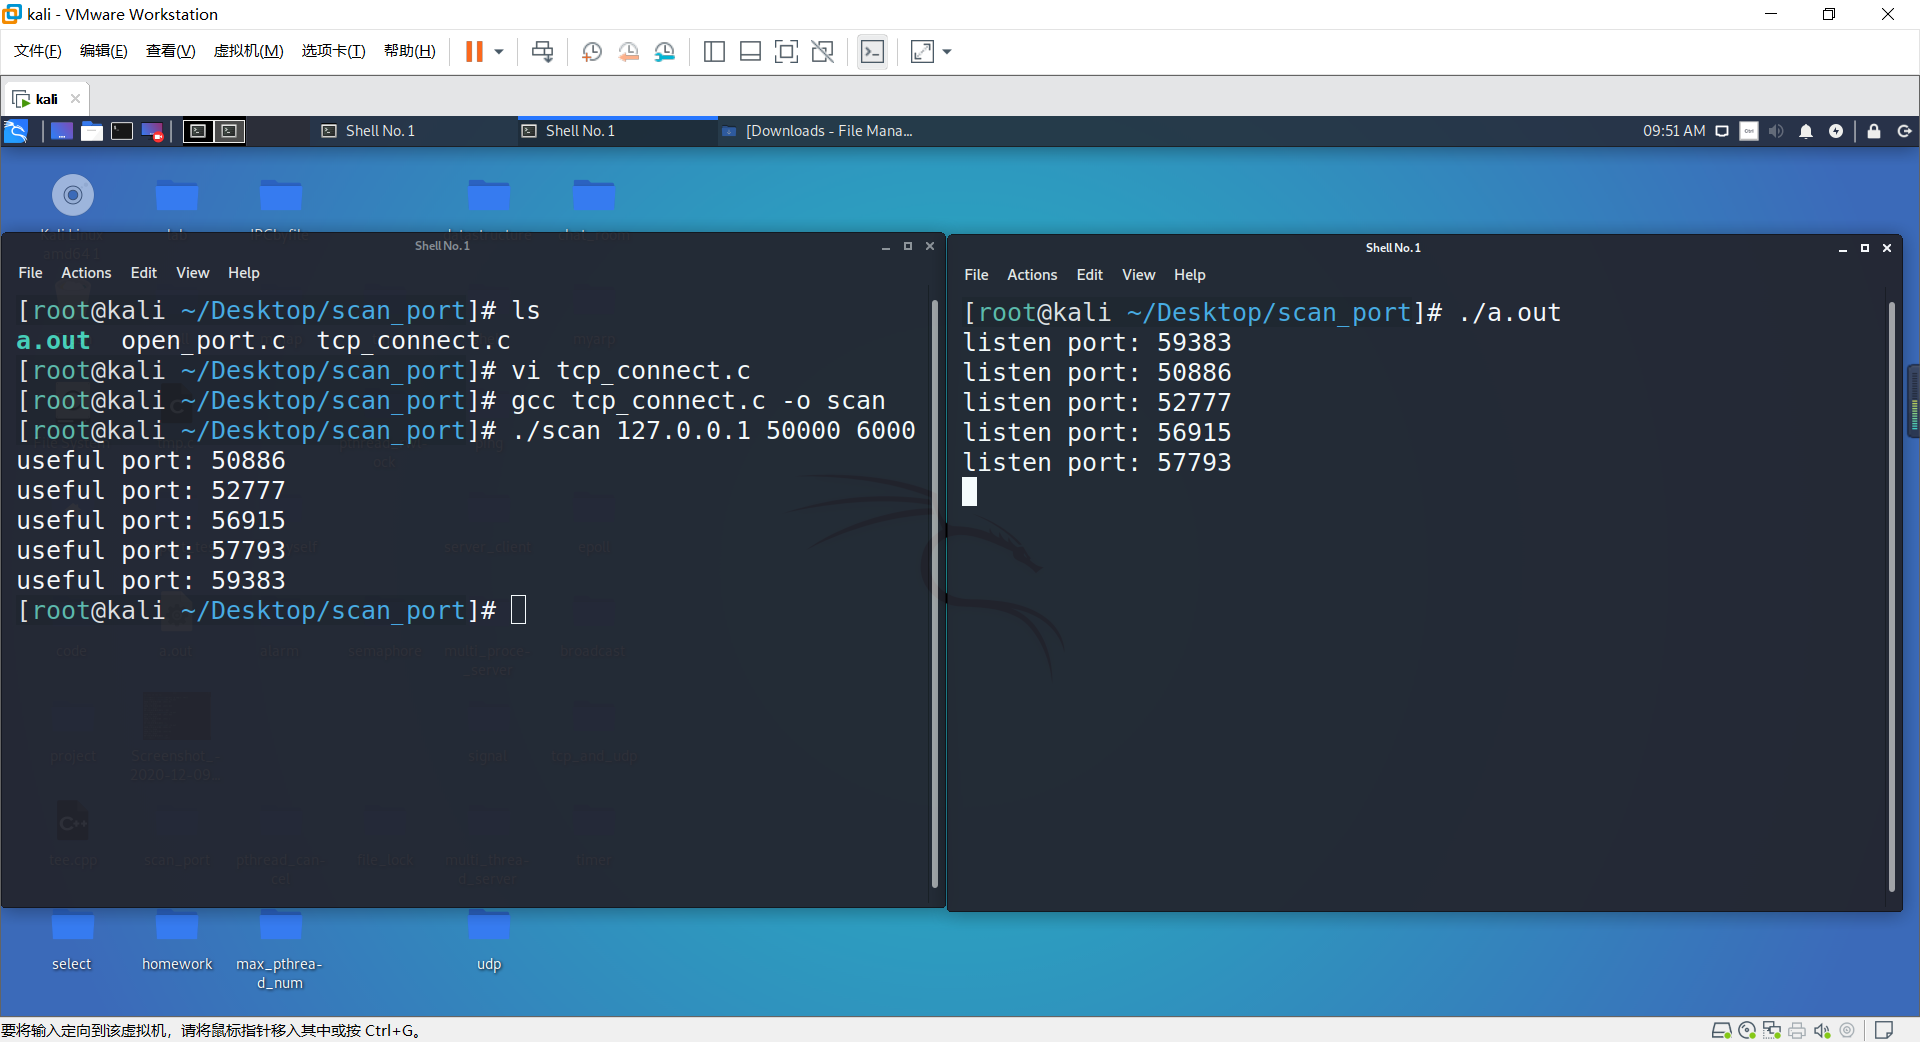
\includegraphics[width=16cm,height=8.7cm]{./figure/25.png}
\end{figure}
\qquad\\
\begin{center}
TCP SYN扫描
\end{center}
SYN扫描就有点难实现了,因为内核封装的接口是实现整个连接,如果只需发送一个同步报文,意味着要自己构建。主要方法包括校验码的计算、报文的发送、报文的接受(因为要判断是不是重置报文)。另外,从\textbf{编程的角度}来说这种方式会比较慢(对比TCP Connect扫描),因为每次都得重新构造一个SYN报文,自行计算检验码,从套接字取得RST报文后进行分析,内核态和用户态切换较频繁。
\begin{lstlisting}[language=C]
#include<stdio.h>
#include<stdlib.h>
#include<errno.h>
#include<sys/socket.h>
#include<arpa/inet.h>
#include<sys/types.h>
#include<linux/tcp.h>
#include<string.h>
#include<netinet/ip.h>
#include<sys/wait.h>
#include<unistd.h>

//计算校验码
unsigned short check_sum(unsigned short *buffer, int size) {
    unsigned long cksum = 0;
    while (size > 1) {
        cksum += *buffer++;
        size -= sizeof (unsigned short);
    }
    if (size) {
        cksum += *(unsigned char*) buffer;
    }
    cksum = (cksum >> 16) + (cksum & 0xffff);
    cksum += (cksum >> 16);

    return (unsigned short) (~cksum);
}

void send_data(int sockfd, struct sockaddr_in *addr, int sourceport, char sourceip[30]) {
    char buffer[100];
    struct iphdr *ip;
    struct tcphdr *tcp;

    int head_len;
    int n, i;
    u_char * pPseudoHead;
    u_char pseudoHead[12 + sizeof (struct tcphdr) ];
    u_short tcpHeadLen;

    tcpHeadLen = htons(sizeof (struct tcphdr));
    head_len = sizeof (struct iphdr) + sizeof (struct tcphdr);
    bzero(buffer, 100);

    //构建ip头
    ip = (struct iphdr *) buffer;
    ip->version = IPVERSION;
    ip->ihl = sizeof (struct ip) >> 2;
    ip->tos = 0;
    ip->tot_len = htons(head_len);
    ip->id = 0;
    ip->frag_off = 0;
    ip->ttl = MAXTTL;
    ip->protocol = IPPROTO_TCP;
    ip->check = 0;
    ip->daddr = addr->sin_addr.s_addr;
    ip->saddr = inet_addr(sourceip);


    //构建TCP头
    tcp = (struct tcphdr *) (buffer + sizeof (struct ip));
    tcp->source = htons(sourceport);
    tcp->dest = addr->sin_port;
    tcp->seq = htonl(30000);
    tcp->ack_seq = 0;
    tcp->doff = 5;
    tcp->syn = 1;
    tcp->urg_ptr = 0;
    tcp->window = htons(10052);


    //构建伪首部
    pPseudoHead = pseudoHead;
    memset(pPseudoHead, 0, 12 + sizeof (struct tcphdr));
    memcpy(pPseudoHead, &ip->saddr, 4);
    pPseudoHead += 4;
    memcpy(pPseudoHead, &ip->daddr, 4);
    pPseudoHead += 4;
    memset(pPseudoHead, 0, 1);
    pPseudoHead++;
    memset(pPseudoHead, 0x0006, 1);
    pPseudoHead++;
    memcpy(pPseudoHead, &tcpHeadLen, 2);
    pPseudoHead += 2;
    memcpy(pPseudoHead, tcp, sizeof (struct tcphdr));

    tcp->check = 0;
    tcp->check = check_sum((unsigned short *) pseudoHead, sizeof (struct tcphdr) + 12);
    if (sendto(sockfd, buffer, head_len, 0, (struct sockaddr *) addr, (socklen_t)sizeof (struct sockaddr_in)) < 0) {
        perror("sendto");
    }
}

void  recv_packet(const char* localIP, int localPort, int sockfd, int startport, int endport) {
    struct tcphdr * tcp;
    char *srcaddr;
    int loopend;
    int size;
    char readbuff[1600];
    struct sockaddr_in from;
    int from_len,n;

    tcp = (struct tcphdr *) (readbuff + 20); /*那个sockfd中读出的数据包括了IP头的所以+20*/
    for (n = startport; n < endport + 1; n++) {
        size = recv(sockfd, readbuff, 1600, MSG_DONTWAIT);
        if (size < (20 + 20))/*读出的数据小于两个头的最小长度的话continue*/
        continue;
        if (ntohs(tcp->dest) != localPort)
        continue;
        if (tcp->rst && tcp->ack)/*端口关闭或者没有服务*/
        continue;
        if (tcp->ack && tcp->syn)/*端口开启*/ {
            printf("%5u open\n", (ntohs(tcp->source)));
            fflush(stdout);
            continue;
        }
    }
}
int main(int argc, char** argv){
    if(argc!=4){
        return -1;
    }
    char ip[30];
    int myport = 8888;
    char* myip = "192.168.145.128";
    int flag = 1;
    strcpy(ip,argv[1]);
    int startport = atoi(argv[2]);
    int endport = atoi(argv[3]);
    struct sockaddr_in addr;
    bzero(&addr,sizeof(addr));
    addr.sin_family = AF_INET;
    inet_pton(AF_INET,ip,&addr.sin_addr);
    int sockfd = socket(AF_INET,SOCK_RAW,IPPROTO_TCP);
    setsockopt(sockfd,IPPROTO_IP,IP_HDRINCL,&flag,sizeof(flag));
    for(int i=startport; i<=endport; ++i){
        addr.sin_port = htons(i);
        send_data(sockfd,&addr,myport,myip);
        recv_packet(myip,myport,sockfd,startport,endport);
    }
    return 0;
}
\end{lstlisting}
\begin{figure}[H]
    \centering
    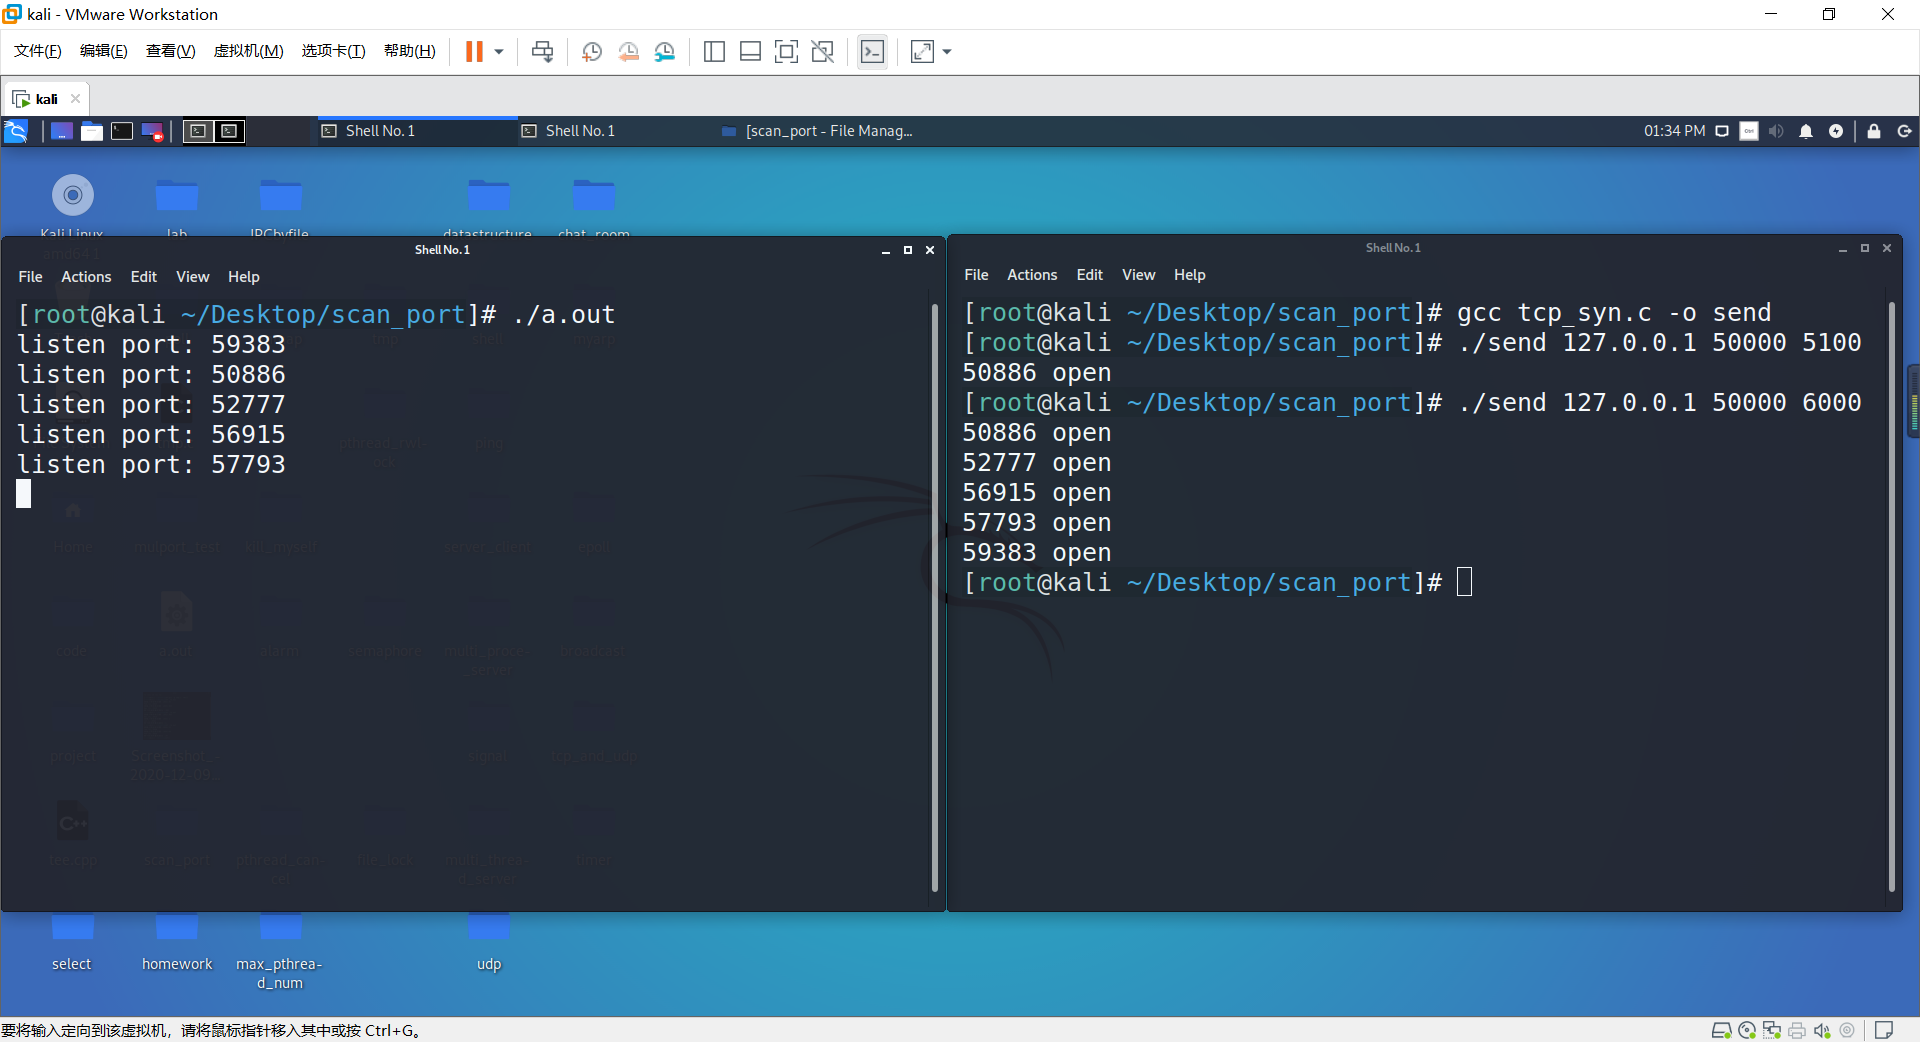
\includegraphics[width=16cm,height=8.7cm]{./figure/27.png}
\end{figure}
\begin{center}
TCP UDP扫描
\end{center}
给一个未开放UDP协议的端口写数据会收到ICMP错误报文,我试了一下资料里介绍的,使用recvfrom函数、sendto函数、write函数进行测试都没有成功,关掉防火墙后也依然没有成功。
\begin{lstlisting}[language=C]
#include<stdio.h>
#include<unistd.h>
#include<string.h>
#include<sys/socket.h>
#include<sys/types.h>
#include<netinet/in.h>
#include<arpa/inet.h>
#include<stdlib.h>
#include<errno.h>
#include<fcntl.h>

const int myport = 8888;
const char* myip = "192.168.145.128";

int main(int argc, char** argv){
    if(argc != 4){
        return -1;
    }
    int flag = 1;
    char dstip[30];
    strcpy(dstip,argv[1]);
    int startport = atoi(argv[2]);
    int endport = atoi(argv[3]);

    int sockfd = socket(AF_INET,SOCK_DGRAM,0);
    /*
    int fl = fcntl(sockfd,F_GETFL,0);
    fcntl(sockfd,F_SETFL,fl|O_NONBLOCK);
    */
    struct sockaddr_in servaddr, cliaddr;
    bzero(&servaddr,sizeof(servaddr));
    bzero(&cliaddr,sizeof(cliaddr));

    servaddr.sin_family = AF_INET;
    inet_pton(AF_INET,dstip,&servaddr.sin_addr);
    const char* string = "hello";
    char buf[BUFSIZ];
    for(int i=startport; i<=endport; ++i){
        servaddr.sin_port = htons(i);
        flag = 1;
        for(int j=0 ;j<3; ++j){
            //int ret = sendto(sockfd,string,strlen(string),0,(struct sockaddr*)&servaddr,sizeof(servaddr));
            int ret = write(sockfd,string,strlen(string));
            if(ret<0){
                flag = 0;
                break;
            }
        }
        if(flag){
            printf("open port: %d\n",i);
        }
        /*
        int len = sizeof(servaddr);
        int ret = recvfrom(sockfd,buf,BUFSIZ,MSG_DONTWAIT,(struct sockaddr*)&servaddr,&len); 
        if(errno!=EAGAIN){
            printf("open port: %d\n",i);
        }
        */
    }
    return 0;
}
\end{lstlisting}
\begin{figure}[H]
    \centering
    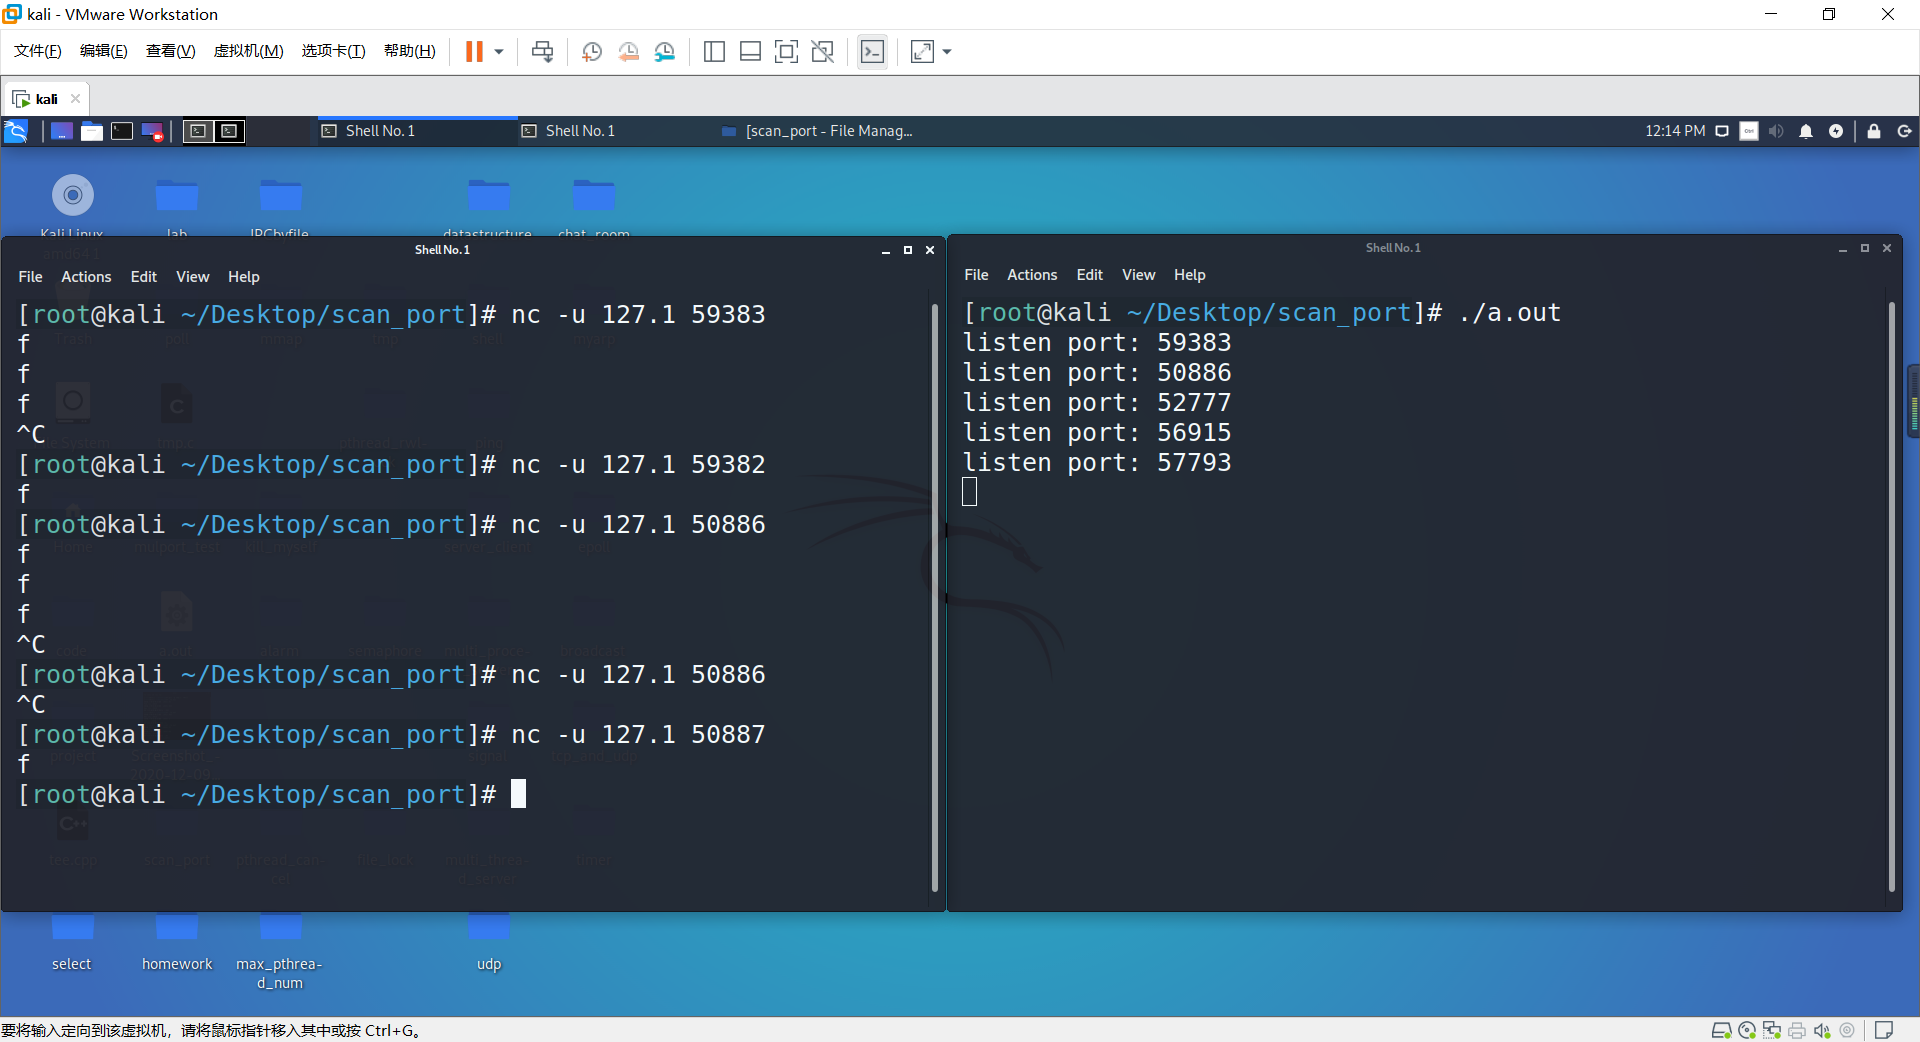
\includegraphics[width=16cm,height=8.7cm]{./figure/26.png}
\end{figure}
不过,在命令行界面访问未开放的UDP端口,可见写入数据时会自动返回,猜想应该是系统收到了ICMP错误报文给进程发送了终止信号。所以有一点可以肯定,向未开放的UDP端口发送数据一定会收到错误报文,但使用系统调用,诸如write、sendto、recvfrom等并不一定能检测。
\end{document}
